%!TEX root=../../main.tex

%\begin{doublespace}
%\begin{spacing}{1.5}

\chapter{Foundations for inference}
\label{foundationsForInference}

\begin{comment}

Have not included using p-values as a measure of the strength of evidence

\end{comment}

Not surprisingly, many studies are now demonstrating the adverse effect of obesity on health outcomes. A 2017 study conducted by the consortium studying the global burden of disease estimates that high body mass index (a measure of body fat that adjusts for height and weight) may account for as many as 4.0 million deaths globally.\footnote{DOI: 10.1056/NEJMoa1614362}  In addition to the physiologic effects of being overweight, other studies have shown that perceived weight status (feeling that one is overweight or underweight) may have a significant effect on self-esteem.\footnote{J Ment Health Policy Econ. 2010 Jun;13(2):53-63}\textsuperscript{,}\footnote{DOI: 10.1186/1471-2458-7-80}  

As stated in its mission statement, the United States Centers for Disease Control and Prevention (US CDC) "serves as
the national focus for developing and applying disease prevention and control, environmental health, and health
promotion and health education activities designed to improve the health of the people of the United
States".\footnote{\url{https://www.cdc.gov/maso/pdf/cdcmiss.pdf}} Since it is not feasible to measure the health
status and outcome of every single US resident, the CDC estimates features of health from samples taken from the population, via large surveys that are repeated periodically. These surveys include the National Health Interview Survey
(NHIS), the National Health and Nutrition Examination Survey (NHANES), the Youth Risk Behavior Surveillance System (YRBSS) and the Behavior Risk Factor Surveillance System (BRFSS).  In the language of statistics, the average weight of all US adults is a \term{population parameter}; the mean weight in a sample or survey is an \term{estimate} of population average weight.  The principles of statistical inference provide not only estimates of population parameters, but also measures of uncertainty that account for the fact that different random samples will produce different estimates because of the variability of random sampling; i.e., two different random samples will not include exactly the same people.

\begin{comment}

There are many parameters of a population that might be of interest in addition to the mean of a variable, such as a median, and might include measures of variability such as a standard deviation or interquartile range.  Population parameters may also include features of categorical variables, such the proportion of a population that feels its current health is only fair or poor.  

\end{comment}

This chapter introduces the important ideas in drawing estimates from samples by discussing methods of inference for a population mean, $\mu$, including three widely used tools: point estimates for a population mean, interval estimates that include both a point estimate and a margin of error, and a method for testing scientific hypotheses about $\mu$. The concepts used in this chapter will appear throughout the rest of the book, which discusses inference for other settings. While particular equations or formulas may change to reflect the details of a problem at hand, the fundamental ideas will not. 

\index{data!cdc|(}

% remember to add closing index indicator

The BRFSS was established in 1984 in 15 states to collect data using telephone interviews about health-related risk behaviors, chronic health conditions. and the use of preventive services.  It now collects data in all 50 states and the District of Columbia from more than 400,000 interviews conducted each year.  The data set \data{cdc} contains a small number of variables from a random sample of 20,000 responses from the 264,684 interviews from the BRFSS conducted in the year 2000.  Part of this dataset is shown in Table~\ref{cdcDF}, with the variables described in Table~\ref{cdcVariables}.\footnote{With small modifications (character strings re-coded as factors), the data appears in this text as it does in an \textit{OpenIntro} lab. \url{http://htmlpreview.github.io/?https://github.com/andrewpbray/oiLabs-base-R/blob/master/intro\_to\_data/intro\_to\_data.html} }



% latex table generated in R 3.3.2 by xtable 1.8-2 package
% Thu Jul  6 08:04:21 2017
\begin{table}[ht]
\centering
\begin{tabular}{rrrlrrrl}
  \hline
 & case & age & gender & weight & wtdesire & height & genhlth \\ 
  \hline
1 &   1 &  77 & m & 175 & 175 &  70 & good \\ 
  2 &   2 &  33 & f & 125 & 115 &  64 & good \\ 
  3 &   3 &  49 & f & 105 & 105 &  60 & good \\ 
  20000 & 20000 &  83 & m & 170 & 165 &  69 & good \\ 
   \hline
\end{tabular}
\caption{Four cases from the \data{cdc} dataset.}
\label{cdcDF}
\end{table}

\begin{table}[h]
\centering\small
\begin{tabular}{l p{110mm}}
\hline
{\bf Variable} & {\bf Variable definition.} \\
\hline
\var{case} & Case number in the dataset, ranging from 1 to 20,000.\\
\var{age} & Age in years. \\
\var{gender} &  A factor variable, with levels \texttt{m} for male, \texttt{f} for female.\\
\var{weight} & Weight in pounds. \\
\var{wtdesire} & Weight that the respondent wishes to be, in pounds. \\
\var{height} & Height in inches. \\
\var{genhlth} & A factor variable describing general health status, with levels \texttt{excellent}, \texttt{very good}, \texttt{good}, \texttt{fair}, \texttt{poor}. \\
\hline
\end{tabular}
\caption{Some variables and their descriptions for the \data{cdc} data set.}
\label{cdcVariables}
\end{table}

Few studies are as large as the original BRFSS dataset (more than 250,000 cases); in fact, few are as large as the 20,000 cases in the dataset \data{cdc}. The dataset \data{cdc} is large enough that estimates calculated from \data{cdc} can be thought of as essentially equivalent to the population characteristics of the entire US adult population. This chapter uses a random sample of 60 cases from \data{cdc}, stored as \data{cdc.samp}, to illustrate the effect of sampling variability and the ideas behind inference. In other words, suppose that \data{cdc} represents the population, and that \data{cdc.samp} is a sample from the population; the goal is to estimate characteristics of the population of 20,000 using only the data from the 60 individuals in the sample.

\begin{comment}

Histograms showing the distributions of height, age, weight, and desired weight in \data{cdc.samp} are shown in Figure~\ref{cdcSampHistograms}

\begin{figure}[h]
\centering
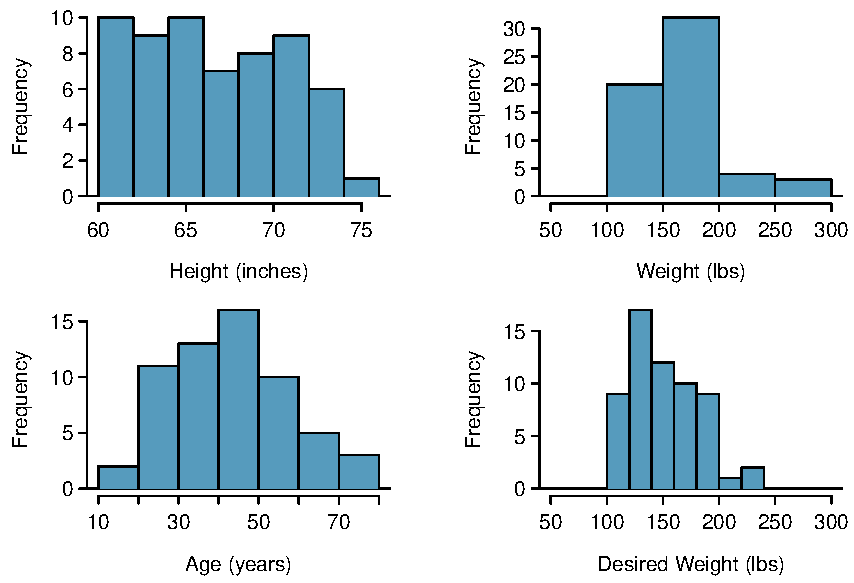
\includegraphics[width=0.8\textwidth]
{ch_inference_foundations_oi_biostat/figures/cdcSampHistograms/cdcSampHistograms} 
\caption{Histograms of \var{height}, \var{age}, \var{weight}, and \var{wtdesire} for the sample data (\data{cdc.samp}).}
\label{cdcSampHistograms}
\end{figure}

\end{comment}

%__________________
\section[Variability in estimates]{Variability in estimates} %\sectionvideohref{youtube-DNIauUrRIEM&list=PLkIselvEzpM7Pjo94m1e7J5jkIZkbQAl4}}
\label{variabilityInEstimates}

\index{point estimate|(}

A natural way to estimate features of the population, such as the population mean weight, is to use the corresponding summary statistic calculated from the sample.\footnote{Other population parameters, such as population median or population standard deviation, can also estimated using sample versions.} The mean weight in the sample of 60 adults in \data{cdc.samp} is $\overline{x}_{\text{weight}} = 173.3$ lbs; this sample mean is a \term{point estimate} of the population mean, $\mu_{\text{weight}}$. If a different random sample of 60 individuals were taken from \data{cdc}, the new sample mean would likely be different as a result of \term{sampling variation}. While estimates generally vary from one sample to another, the population mean is a fixed value.  

\begin{comment}

Other population parameters, such as population median or population standard deviation, can also estimated using sample versions. The median weight in the sample of 60 adults is 165lbs, reflecting the right-skewed distribution for weight visible in Figure~\ref{cdcSampHistograms}.  The boxplot of weight in the sample (Figure~\ref{cdcSampWeightBoxPlot}) shows more clearly the reason for the difference between the mean and the median.  There are outliers above the third quartile, recorded weights of 290, 300 and 400 lbs. These are indeed large weights, but with the increase prevalence of obesity in the United States, they are not impossibly large and will not be eliminated from the sample.

\begin{figure}
\centering
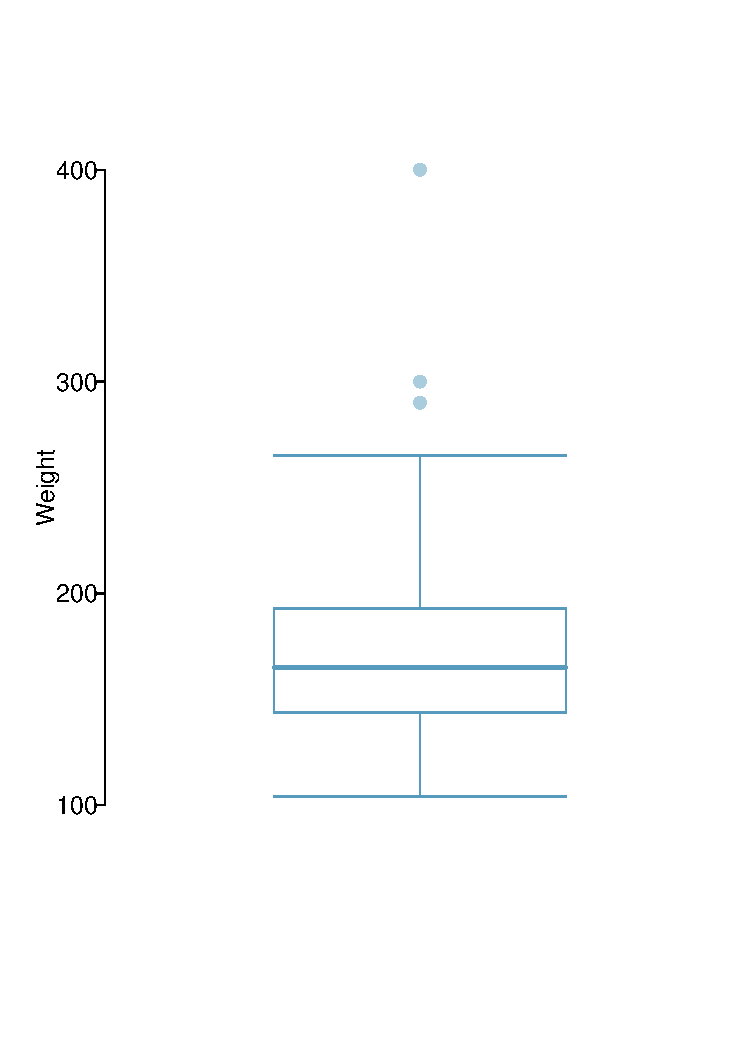
\includegraphics[width=0.8\textwidth]
{ch_inference_foundations_oi_biostat/figures/cdcSampWeightBoxPlot/cdcSampWeightBoxPlot.pdf} 
\caption{Histograms of \var{height}, \var{age}, \var{weight}, and \var{wtdesire} for the sample data (\data{cdc.samp}).}
\label{cdcSampHistograms}
\end{figure}

\end{comment}

\begin{exercise} \label{peOfDiffWeightBetweenGender}
	How would one estimate the difference in average weight between men and women? Given that $\overline{x}_{\text{men}} = 185.1$ lbs and $\overline{x}_{\text{women}} = 162.3$ lbs, what is a good point estimate for the population difference?\footnote{Given that $\overline{x}_{\text{men}} = 185.1$ lbs and $\overline{x}_{\text{women}} = 162.3$ lbs, the difference of the two sample means, $185.1 - 162.3 = 22.8$lbs, is a point estimate of the difference. The data in the random sample suggests that adult males are, on average, about 23~lbs heavier than adult females.}
\end{exercise}

Point estimates become more accurate with increasing sample size. Figure~\ref{cdcWeightRunningMean} shows the sample mean weight calculated for random samples drawn from \data{cdc}, where sample size increases by 1 for each draw until sample size equals 500. The red dashed horizontal line in the figure is drawn at the average weight of all adults in \data{cdc}, 169.7 lbs, which represents the population mean weight.\footnote{It is not exactly the mean weight of all US adults, but will be very close since \data{cdc} is so large.}

\begin{figure}[h]
	\centering
	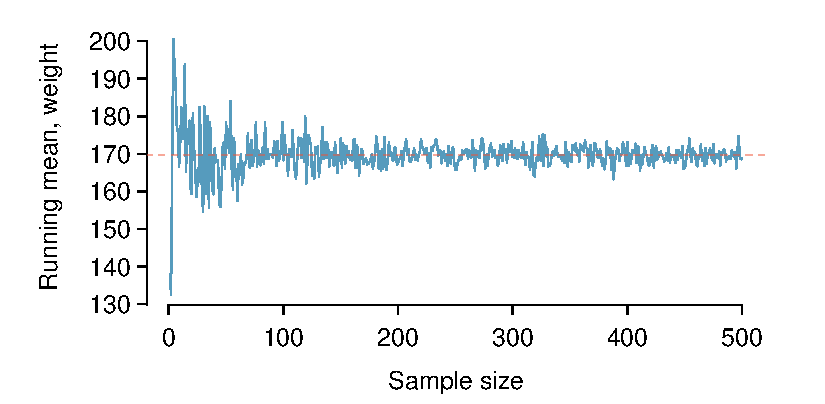
\includegraphics[width=0.95\textwidth]{ch_inference_foundations_oi_biostat/figures/cdcWeightRunningMean/cdcWeightRunningMeanNew.pdf}
	\caption{The mean \var{weight} computed for a random sample from \data{cdc}, increasing sample size one at a time until $n = 500$. The sample mean approaches the population mean (i.e., mean weight in \data{cdc}) as sample size increases.}
	\label{cdcWeightRunningMean}
\end{figure}

Note how a sample size around 50 may produce a sample mean that is as much as 10 lbs higher or lower than the population mean. As sample size increases, the fluctuations around the population mean decrease; in other words, as sample size increases, the sample mean becomes less variable and provides more reliable estimate of the population mean.

%JV: with the edits, this figure no longer shows a 'running mean'.


\subsection{The sampling distribution for the mean}

The sample mean weight calculated from \data{cdc.samp} is 173.3~lbs. Another random sample of 60 participants might produce a different value of $\overline{x}$, such as 169.5~lbs; repeated random sampling could result in additional different values, perhaps 172.1~lbs, 168.5~lbs, and so on. Each sample mean $\overline{x}$ can be thought of as a single observation from a random variable $\overline{X}$. The distribution of $\overline{X}$ is called the \term{sampling distribution of the sample mean}, and has its own mean and standard deviation like the random variables discussed in Chapter 3. The concept of a sampling distribution can be illustrated by taking repeated random samples from \data{cdc}. Figure~\ref{cdcWeight1000SampDist} shows a histogram of sample means from 1,000 random samples of size 60 from \data{cdc}. The histogram provides an approximation of the theoretical sampling distribution of $\overline{X}$ for samples of size 60. 

\begin{figure}[h]
	\centering
	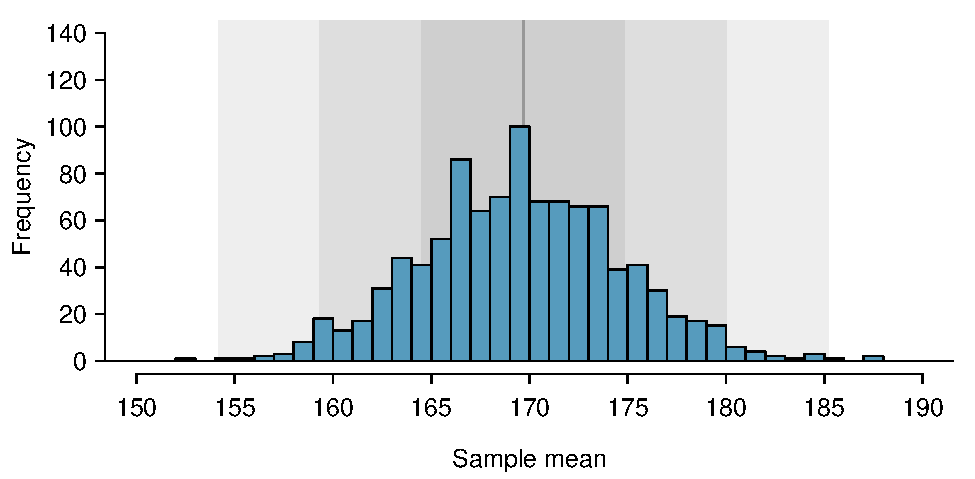
\includegraphics[width=0.9\textwidth]
	{ch_inference_foundations_oi_biostat/figures/cdcWeight1000SampDist/cdcWeight1000SampDist}
	\caption{A histogram of 1000 sample means for weight among US adults, where the samples are of size $n=60$.}
	\label{cdcWeight1000SampDist}
\end{figure}

\begin{termBox}{\tBoxTitle{Sampling distribution}
The sampling distribution is the distribution of the point estimates based on samples of a fixed size from a certain population. It is useful to think of a particular point estimate as being drawn from a sampling distribution.}
\end{termBox}

Since the complete sampling distribution consists of means for all possible samples of size 60, drawing a much larger number of samples provides a more accurate view of the distribution; the left panel of Figure~\ref{cdcWeightBigSampDist} shows the distribution calculated from 100,000 sample means. 

\begin{figure}[hht]
 	\centering
 	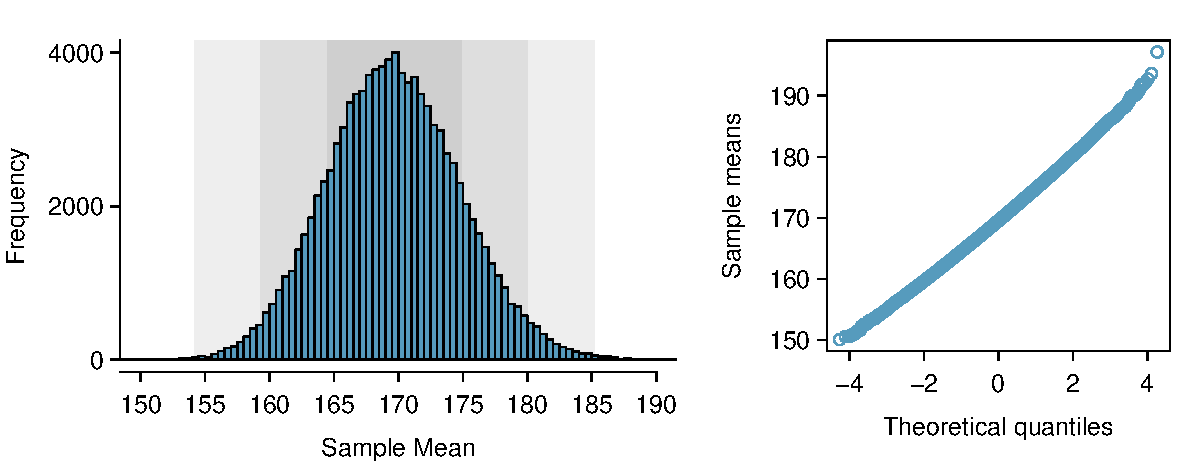
\includegraphics[width=\textwidth]
 	{ch_inference_foundations_oi_biostat/figures/cdcWeightBigSampDist/cdcWeightBigSampDist.pdf}
 	\caption{The left panel shows a histogram of the sample means for 100,000 random samples. The right panel shows a normal probability plot of those sample means.}
 	\label{cdcWeightBigSampDist}
\end{figure}
 
A normal probability plot of these sample means is shown in the right panel of Figure~\ref{cdcWeightBigSampDist}. All of the points closely fall around a straight line, implying that the distribution of sample means is nearly normal (see Section~\ref{normalDist}). This result follows from the Central Limit Theorem.
 
 \begin{termBox}{\tBoxTitle{Central Limit Theorem, informal description}
 		If a sample consists of at least 30 independent observations and the data are not strongly skewed, then the distribution of the sample mean is well approximated by a normal model.\index{Central Limit Theorem}}
 \end{termBox}

The sampling distribution for the mean is unimodal and symmetric around the mean of the random variable $\overline{X}$. Statistical theory can be used to show that the mean of the sampling distribution for $\overline{X}$ is exactly equal to the population mean $\mu$. 

However, in almost any study, conclusions about a population parameter must be drawn from the data collected from a single sample. The sampling distribution of $\overline{X}$ is a theoretical concept, since obtaining repeated samples by conducting a study many times is not possible. In other words, it is not feasible to calculate the population mean $\mu$ by finding the mean of the sampling distribution for $\overline{X}$.

\subsection{Standard error of the mean}
\label{seOfTheMean}

The \term{standard error (SE)}\index{SE}\marginpar[\raggedright\vspace{-4mm}

$SE$\\\footnotesize standard\\error]{\raggedright\vspace{-4mm}

$SE$\\\footnotesize standard\\error} of the sample mean measures the sample-to-sample variability of $\overline{X}$, the extent to which values of the repeated sample means oscillate around the population mean. The theoretical standard error of the sample mean is calculated by dividing the population standard deviation ($\sigma_{x}$) by the square root of the sample size $n$. Since the population standard deviation $\sigma$ is typically unknown, the sample standard deviation $s$ is often used in the definition of a standard error; $s$ is a reasonably good estimate of $\sigma$. If $\overline{x}$ is the sample mean weight, its standard error (denoted by SE) is
\[\text{SE}_{\overline{x}} = \dfrac{s_{x}}{\sqrt{n}} = \dfrac{49.04}{\sqrt{60}} = 6.33. \]

This estimate tends to be sufficiently good when the sample size is at least 30 and the population distribution is not strongly skewed. In the case of skewed distributions, a larger sample size is necessary.

The probability tools of Section~\ref{randomVariablesSection} can be used to derive the formula $\sigma_{\overline{X}} = \sigma_x/\sqrt{n}$, but the derivation is not shown here. Larger sample sizes produce sampling distributions that have lower variability. Increasing the sample size causes $\overline{X}$ to be clustered more tightly around the population mean $\mu$, allowing for more accurate estimates of $\mu$ from a single sample, as shown in Figure~\ref{cdcSamplingVariabilityComparison}. When sample size is large, it is more likely that any particular sample will have a mean close to the population mean. 

\begin{figure}[h!]
	\centering
	\subfigure[]{
		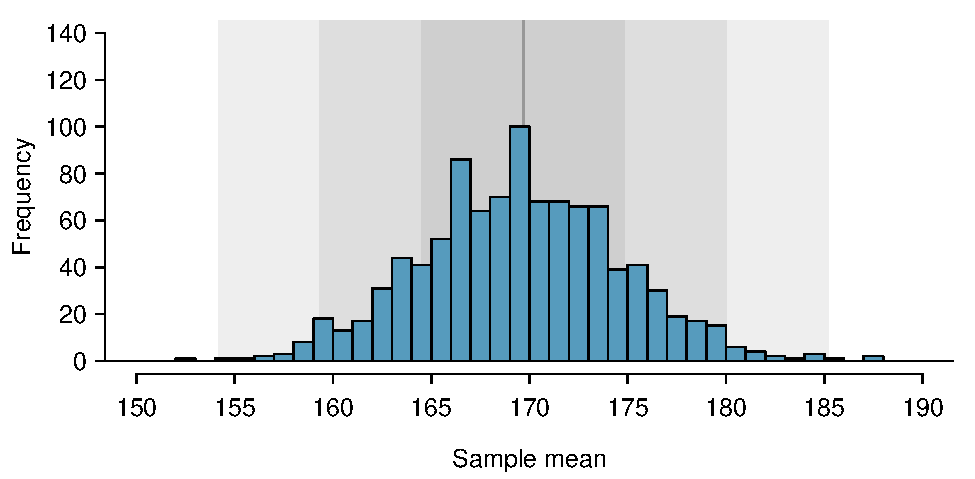
\includegraphics[width=0.46\textwidth]{ch_inference_foundations_oi_biostat/figures/cdcWeight1000SampDist/cdcWeight1000SampDist}
		\label{cdcWeight1000SampDistA}
	}
	\subfigure[]{
		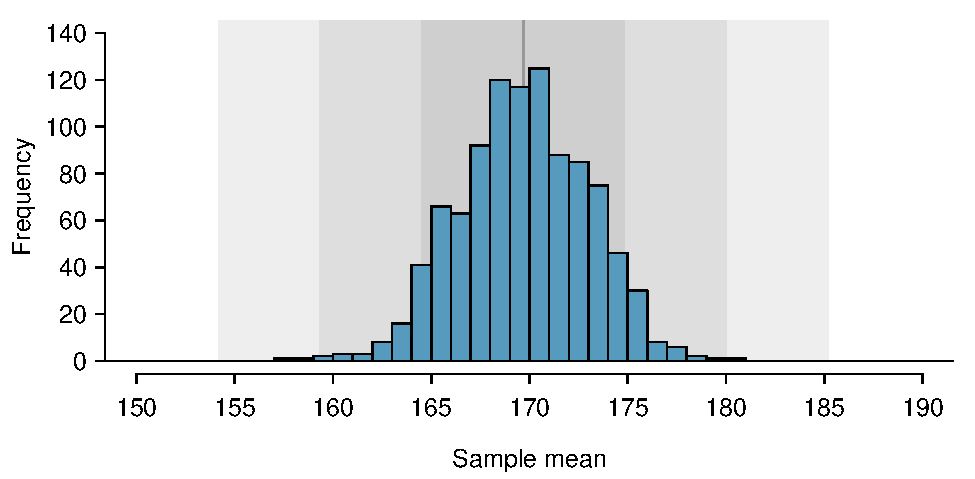
\includegraphics[width=0.46\textwidth]{ch_inference_foundations_oi_biostat/figures/cdcWeight1000SampDist/cdcWeight1000SampDistB} 
		\label{cdcWeight1000SampDistB}		
	}
	\caption{\subref{cdcWeight1000SampDistA} Reproduced from Figure~\ref{cdcWeight1000SampDist}, an approximation of the sampling distribution of $\overline{X}$ with $n = 60$. \subref{cdcWeight1000SampDistB} An approximation of the sampling distribution of $\overline{X}$ with $n = 200$.}
	\label{cdcSamplingVariabilityComparison}
\end{figure}


\begin{termBox}{\tBoxTitle{The standard error (SE) of the sample mean}
		Given $n$ independent observations from a population with standard deviation $\sigma$, the standard error of the sample mean is equal to \vspace{-1mm}
		\begin{align*}
          \text{SE}_{\overline{x}} = \frac{s_x}{\sqrt{n}}.
		\label{seOfXBar}
		\end{align*}\vspace{-3mm}%
		
        This is an accurate estimate of the theoretical standard deviation of $\overline{X}$ when the sample size is at least 30 and the population distribution is not strongly skewed.}
\end{termBox}

\begin{termBox}{\tBoxTitle{Summary: Point estimate terminology}
\begin{itemize}
	\setlength{\itemsep}{0mm}	
	\item The population mean and standard deviation are denoted by $\mu$ and $\sigma$. 
	
	\item The sample mean and standard deviation are denoted by $\overline{x}$ and $s$. 
	
	\item The distribution of the random variable $\overline{X}$ refers to the collection of sample means if multiple samples of the same size were repeatedly drawn from a population. 
	
	\item The mean of the random variable $\overline{X}$ equals the population mean $\mu$.  In the notation of Chapter~\ref{modeling}, $\mu_{\overline{X}} = E(\overline{X}) = \mu$.
	
	\item  The standard deviation of $\overline{X}$ ($\sigma_{\overline{X}})$ is called the standard error (SE) of the sample mean $\overline{x}$. 
	
	\item The theoretical standard error of the sample mean, as calculated from a single sample of size $n$, is equal to $\frac{\sigma}{\sqrt{n}}$. The standard error is abbreviated by SE and is usually estimated by using $s$, the sample standard deviation, such that $SE = \frac{s}{\sqrt{n}}$.
	
\end{itemize}
	}
\end{termBox}

\index{point estimate|)}

\section[Confidence intervals]{Confidence intervals}
\label{confidenceIntervals}
\subsection{Interval estimates for a population parameter}

While a point estimate consists of a single value, an interval estimate provides a plausible range of values for a parameter. When estimating a population mean $\mu$, a \term{confidence interval} for $\mu$ has the general form
\[(\overline{x} -m, \ \overline{x} + m) = \overline{x} \pm m, \]
where $m$ is the \term{margin of error}. Intervals that have this form are called \term{two-sided confidence intervals} because they provide both lower and upper bounds, $\overline{x} - m$ and $\overline{x} + m$, respectively. One-sided sided intervals are discussed in Section~\ref{onesidedCIs}.

The standard error of the sample mean is the standard deviation of its distribution; additionally, the distribution of sample means is nearly normal and centered at $\mu$. Thus, under the normal model, the sample mean $\overline{x}$ will be within 1.96 standard errors (i.e., standard deviations) of the population mean $\mu$ approximately 95\% of the time.\footnote{In other words, the $Z$-score of 1.96 is associated with 2.5\% area to the right (and $Z$ = -1.96 has 2.5\% area to the left); this can be found on normal probability tables or from using statistical software.} Thus, if an interval is constructed that spans 1.96 standard errors from the point estimate in either direction, a data analyst can be 95\% \term{confident} that the interval

\begin{align}
  \overline{x}\ \pm\ 1.96\times \text{SE} 
\label{95PercentCIWhenUsingNormalModel}
\end{align}

contains the population mean. The value 95\% is an approximation, accurate when the sampling distribution for the sample mean is close to that of a normal distribution. This assumption holds when the sample size is sufficiently large (guidelines for `sufficiently large' are given in Section~\ref{ch4Summary}).

\begin{figure}[h!]
	\centering
	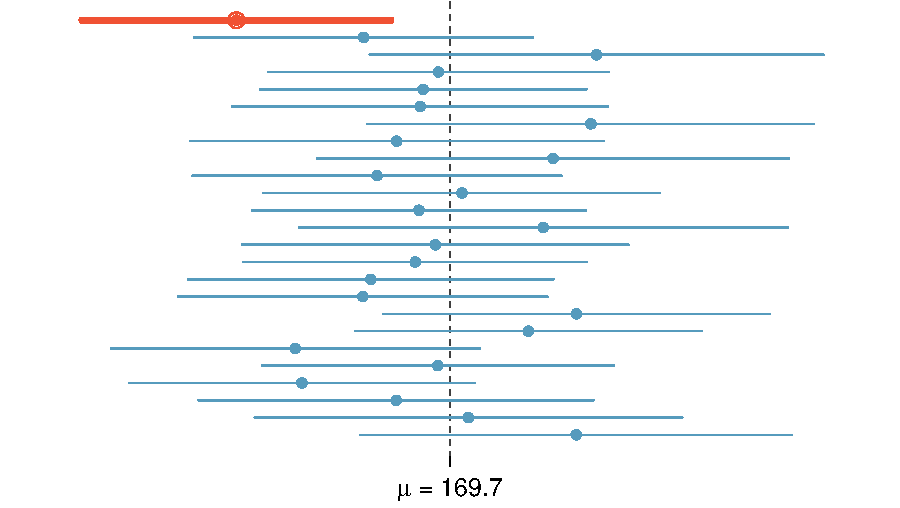
\includegraphics[width=0.70\textwidth]
	{ch_inference_foundations_oi_biostat/figures/95PercentConfidenceInterval/95PercentConfidenceInterval.pdf}
	\caption{Twenty-five samples of size $n=60$ were taken from \data{cdc}. For~each sample, a 95\% confidence interval was calculated for the population average adult weight. Only~1 of these~25 intervals did not contain the population mean, $\mu = 169.7$~lbs.}
	\label{95PercentConfidenceInterval}
\end{figure}

The phrase "95\% confident" has a subtle interpretation: if many samples were drawn from a population, and a confidence interval is calculated from each one using Equation~\ref{95PercentCIWhenUsingNormalModel}, about 95\% of those intervals would contain the population mean $\mu$. Figure~\ref{95PercentConfidenceInterval} illustrates this process with 25 samples taken from \data{cdc}. Of the 25 samples, 24 contain the mean weight in \data{cdc} of 169.7 lbs, while one does not. 

Just as with the sampling distribution of the sample mean, the interpretation of a confidence interval relies on the abstract construct of repeated sampling. A data analyst, who can only observe one sample, does not know whether the population mean lies within the single interval calculated. The uncertainty is due to random sampling\textemdash by chance, it is possible to select a sample from the population that has unusually high (or low) values, resulting in a sample mean $\overline{x}$ that is relatively far from $\mu$, and by extension, a confidence interval that does not contain $\mu$. 

\begin{example}{The sample mean adult weight from the 60 observations in \data{cdc.samp} is $\overline{x}_{\text{weight}} = 173.3$~lbs, and the standard deviation is $s_{\text{weight}} = 49.04$~lbs.  Use Equation~\ref{95PercentCIWhenUsingNormalModel} to calculate an approximate 95\% confidence interval for the average adult weight in the US population.}
  The standard error for the sample mean is  $\text{SE}_{\overline{x}}=\frac{49.04}{\sqrt{60}} = 6.33$~lbs. The 95\% confidence interval is
 \[\overline{x}_{\text{weight}} \pm 1.96 \text{SE}_{\overline{x}} = 173.3 \pm (1.96)(6.33) = (160.89, 185.71)~\text{lbs.} \]
  
  The data support the conclusion that, with 95\% confidence, the average weight of US adults is between approximately 161 and 186~lbs.
  
  Figure~\ref{cdcWeightBigSampDist} visually shows that the sampling distribution is nearly normal. To assess normality of the sampling distribution without repeated sampling, it is necessary to check whether the data are skewed. Although Figure~\ref{cdcWeightHist} shows some skewing, the sample size is large enough that the confidence interval should be reasonably accurate.
  
  \begin{figure}[h!]
  	\centering
  	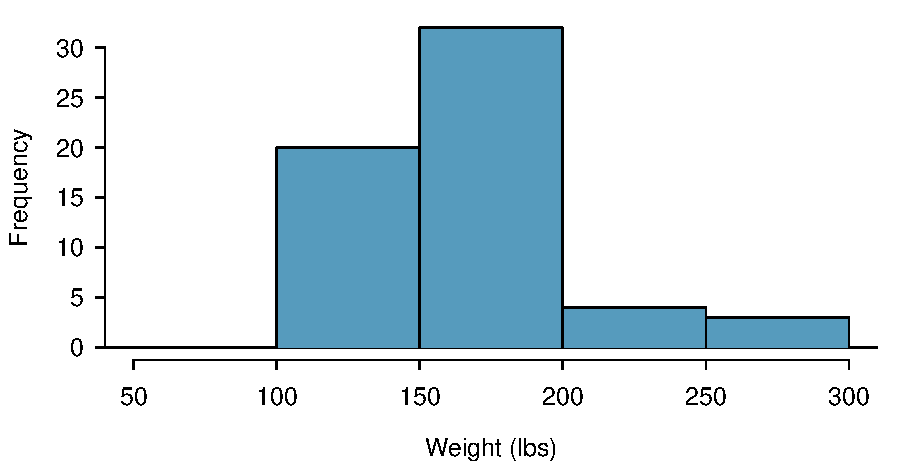
\includegraphics[width=0.55\textwidth]
  	{ch_inference_foundations_oi_biostat/figures/cdcWeightHist/cdcWeightHist.pdf}
  	\caption{Histogram of \var{weight} in \data{cdc.samp} }
  	\label{cdcWeightHist}
  \end{figure}
  
  \end{example}

  \begin{exercise} \label{95CIExerciseForWeightUSFemales}
    The are 31 females in the sample of 60 US adults, and the average and standard deviation of weight for these individuals are 162.3~lbs and 57.74~lbs, respectively.  A histogram of \var{weight} for the 31 females is shown in Figure~\ref{cdcFemaleWeightHist}.  Calculate an approximate 95\% confidence interval for the average weight of US females.  Is the interval likely to be accurate?\footnote{Applying Equation~\ref{95PercentCIWhenUsingNormalModel}: $162.3  \pm (1.96)(57.73/\sqrt{31}) \rightarrow (149.85, 174.67)$.  The usual interpretation would be that a data analyst can be about 95\% confident the average weight of US females is between approximately 150 and 175~lbs.  However, the histogram of female weights shows substantial right skewing, and several females with recorded weights larger than 200~lbs. The confidence interval is probably not accurate; a larger sample should be collected in order for the sampling distribution of the mean to be approximately normal.  Chapter~\ref{inferenceForNumericalData} will introduce the $t$-distribution, which is more reliable with small sample sizes than the $z$-distribution.}
\end{exercise}

\begin{figure}[hht]
   \centering
   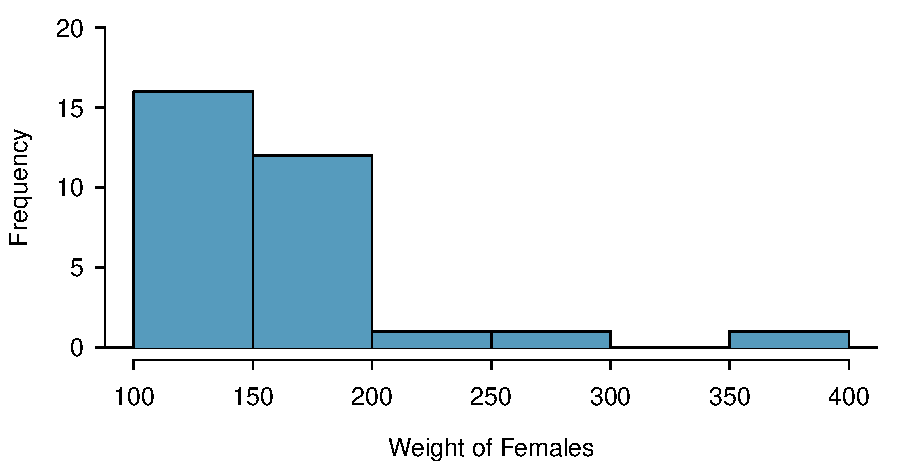
\includegraphics[width=0.5\textwidth]
{ch_inference_foundations_oi_biostat/figures/cdcFemaleWeightHistogram/cdcFemaleWeightHistogram.pdf}
\caption{Histogram of \var{weight} for the 31 females in \data{cdc.samp}.}
\label{cdcFemaleWeightHist}
\end{figure}


\subsection{Changing the confidence level}
\label{changingTheConfidenceLevelSection}

\index{confidence interval!confidence level|(}

Ninety-five percent confidence intervals are the most commonly used interval estimates, but intervals with confidence levels other than 95\% can also be constructed. The general formula for a confidence interval (for the population mean $\mu$) is given by 
\begin{align}
	\overline{x} \pm \ z^{\star} \times \text{SE},
\end{align}
where $z^{\star}$ is chosen according to the confidence level. When calculating a 95\% confidence level, $z^{\star}$ is 1.96, since the area within 1.96 standard deviations of the mean captures 95\% of the distribution.

To construct a 99\% confidence interval, $z^{\star}$ must be chosen such that 99\% of the normal curve is captured between -$z^{\star}$ and $z^{\star}$.

\begin{example}{Let $Y$ be a normally distributed random variable. Ninety-nine percent of the time, $Y$ will be within how many standard deviations of the mean?}
	This is equivalent to the $z$-score with 0.005 area to the right of $z$ and 0.005 to the left of $-z$. In the normal probability table, this is the $z$-value that with 0.005 area to its right and 0.995 area to its left. The closest two values are 2.57 and 2.58; for convenience, round up to 2.58. The unobserved random variable $Y$ will be within 2.58 standard deviations of $\mu$ 99\% of the time, as shown in Figure~\ref{choosingZForCI}.
\end{example}

\begin{figure}[h]
\begin{centering}
	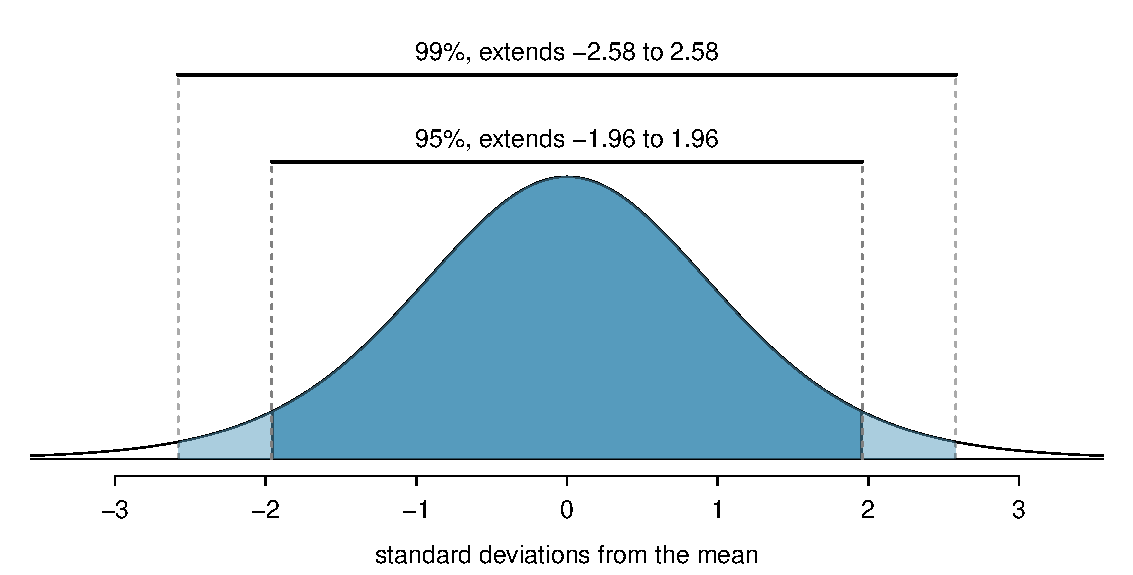
\includegraphics[width=\textwidth]
	{ch_inference_foundations_oi_biostat/figures/choosingZForCI/choosingZForCI.pdf}
	\caption{The area between -$z^{\star}$ and $z^{\star}$ increases as $|z^{\star}|$ becomes larger. If the confidence level is 99\%, $z^{\star}$ is chosen such that 99\% of the normal curve is between -$z^{\star}$ and $z^{\star}$, which corresponds to 0.5\% in the lower tail and 0.5\% in the upper tail: $z^{\star}=2.58$.}
	\label{choosingZForCI}
  \end{centering}
	\index{confidence interval!confidence level|)}
\end{figure}
 
A 99\% confidence interval will have the form 
\begin{align}
	\overline{x} \pm \ 2.58 \times \text{SE},
\end{align}
 and will consequently be wider than a 95\% interval for $\mu$ calculated from the same data, since the margin of error $m$ is larger.


\begin{comment}
% WARNING !!!!
% EOCE 4.9 (as of 2nd Edition) references the results of this exercise
\begin{example} {
	Create a 99\% confidence interval for the average days active per week of all YRBSS students using \data{yrbss.samp}. The point estimate is $\overline{x}_{active} = 3.93$ and the standard error is $SE_{\overline{x}} = 0.25$.}
Apply the 99\% confidence interval formula: $\overline{x}_{active}\ \pm\ 2.58 \times  SE_{\overline{x}} \rightarrow (3.28, 4.58)$. We are 99\% confident that the average days active per week of all YRBSS students is between 3.28 and 4.58~days.
\end{example}
%library(openintro); data(yrbss.samp); d <- yrbss.samp; mean(d$age); sd(d$age)/sqrt(100)

\end{comment}

\begin{example} {
    Create a 99\% confidence interval for the average adult weight in the US population using the data in \data{cdc.samp}. The point estimate is $\overline{x}_{weight} = 173.3$ and the standard error is $SE_{\overline{x}} = 6.33$.}
Apply the 99\% confidence interval formula: $\overline{x}_{weight}\ \pm\ 2.58 \times  SE_{\overline{x}} \rightarrow (156.97, 189.63)$. A data analyst can be 99\% confident that the average adult weight is between 156.97 and 189.63~lbs.
\end{example}

The 95\% confidence interval for the average adult weight is (160.89, 185.71)~lbs. Increasing the confidence level to 99\% results in the interval (156.97, 189.63) lbs; this wider interval is more likely to contain the population mean $\mu$. However, increasing the confidence level comes at a cost: a wider interval is less informative in providing a precise estimate of the population mean. Consider the extreme: to be "100\% confident" that an interval contains $\mu$, the interval must span all possible values of $\mu$. For example, with 100\% confidence the average weight is between 0 and 1000 lbs; while this interval necessarily contains $\mu$, it has no interpretive value and is completely uninformative.\footnote{Strictly speaking, to be 100\% confident requires an interval spanning all positive numbers; 1000 lbs has been arbitrarily chosen as an upper limit for human weight.} 

Decreasing the confidence level results in a narrower interval and a more precise estimate, but the interval has less chance of containing $\mu$. For example, consider a 50\% confidence interval for average adult weight using \data{cdc.samp}: the $z^{\star}$ value is 0.67, and the confidence interval is (169.06, 177.54)~lbs. This interval provides more precise estimate of the population average weight $\mu$ than the 99\% or 95\% confidence intervals, but there is only a 50\% chance that it contains $\mu$.

The choice of confidence level is a trade-off between obtaining a precise estimate and calculating an interval that likely contains the population parameter. In published literature, the most used confidence intervals are the 90\%, 95\%, and 99\%. 

\subsection{One-sided confidence intervals}
\label{onesidedCIs}

One-sided confidence intervals for a population mean provide either a lower bound or an upper bound, but not both.  One-sided confidence intervals have the form
\[
(\overline{x} - m, \infty) \text{ or } (-\infty, \overline{x} + m).
\]

While the margin of error $m$ for a one-sided interval is still calculated from the standard error of $\overline{x}$ and a $z^\star$ value, the choice of $z^\star$ is a different than for a two-sided interval. For example, the intent of a 95\% one-sided upper confidence interval is to provide an upper bound $m$ such that a data analyst can be 95\% confident that a population mean $\mu$ is less than $\overline{x} + m$. The $z^\star$ value must correspond to the point on the normal distribution that has 0.05 area in the right tail, $z^{\star} = 1.645$.\footnote{Previously, with a two-sided interval, 1.96 was chosen in order to have a total area of 0.05 from both the right and left tails.} A one-sided upper 95\%  confidence interval will have the form
\begin{align*}
(-\infty, \overline{x} + 1.645 \times \text{SE}).
\end{align*}

\begin{example}
  {Calculate a lower 95\% confidence interval for the population average adult weight in the United States. In the sample of 60 adults in \data{cdc.samp}, the mean and standard error are $\overline{x} = 173.3$ and $SE = 6.33$ days.}
	
The lower bound is $173.3 - (1.645 \times 6.33) = 163.89$. The lower 95\% interval $(163.89, \infty)$ suggests that one can be 95\% confident that the population average adult weight is at least 163.9~lbs. 
\end{example}

\begin{exercise} Calculate an upper 99\% confidence interval for the population average adult weight in the United States. The mean and standard error for weight in \data{cdc.samp} are $\overline{x} = 173.3$ and $SE = 6.33$ days.\footnote{For a one-sided 99\% confidence interval, the $z^\star$ value corresponds to the point with 0.01 area in the right tail, $z^\star = 2.326$. Thus, the upper bound for the interval is $173.3 + (2.326 \times 6.33) = 188.024.$ The upper 99\% interval ($-\infty, 188.024$) suggests that one can be 99\% confident that the population average adult weight is at most 188.0 lbs.}
	
\end{exercise}

%JV: Needs explanation about when to use one-sided interval versus two-sided.

\subsection{Interpreting confidence intervals}
\label{interpretingCIs}

\index{confidence interval!interpretation|(}

The correct interpretation of an XX\% confidence interval is, "We are XX\% confident that the population parameter is between \dots" While it may be tempting to say that a confidence interval captures the population parameter with a certain probability, this is a common error. The confidence level only quantifies how plausible it is that the parameter is within the interval; there is no probability associated with whether a parameter is contained in a specific confidence interval. The confidence coefficient reflects the nature of a procedure that is correct XX\% of the time, given that the assumptions behind the calculations are true.

The conditions regarding the validity of the normal approximation can be checked using the numerical and graphical summaries discussed in Chapter 1. However, the condition that data should be from a random sample is sometimes overlooked. If the data are not from a random sample, then the confidence interval no longer has interpretive value, since there is no population mean to which the confidence interval applies. For example, while only simple arithmetic is needed to calculate a confidence interval for BMI from the \data{famuss} dataset in Chapter 1, the participants in the study are almost certainly not a random sample from some population; thus, a confidence interval should not be calculated in this setting.

\begin{example}{Body mass index (BMI) is one measure of body weight that adjusts for height. The National Health and Nutrition Examination Survey (NHANES) consists of a set of surveys and measurements conducted by the US CDC to assess the health and nutritional status of adults and children in the United States. The dataset \data{nhanes.samp} contains 76 variables and is a random sample of 200 individuals from the measurements collected in the years 2009-2010 and 2012-2013.\footnote{The sample was drawn from a larger sample of 20,293 participants in the \textbf{NHANES} package, available from The Comprehensive R Archive Network (CRAN). The CDC uses a complex sampling design that samples some demographic subgroups with larger probabilities, but \data{nhanes.samp} has been adjusted so that it can be viewed as a random sample of the US population.} Use \data{nhanes.samp} to calculate a 95\% confidence interval for adult BMI in the US population, and assess whether the data suggest Americans tend to be overweight. \label{exNhanesBmi}}
	
\begin{figure}[h]
		\centering
		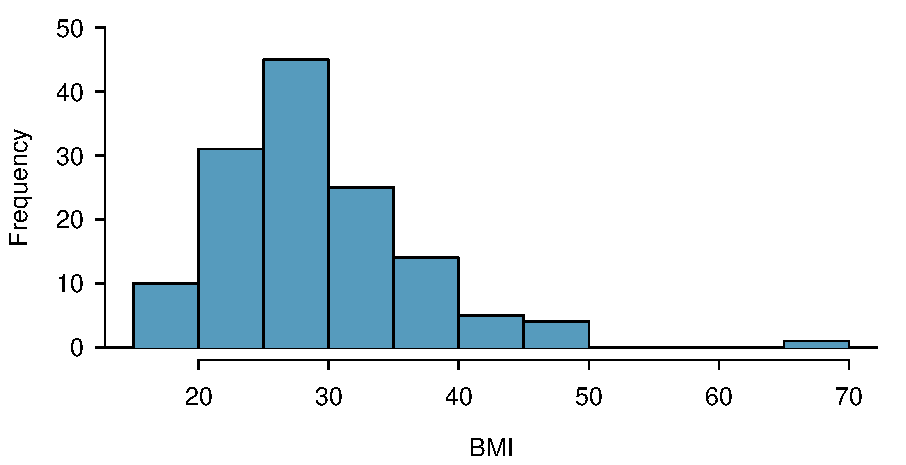
\includegraphics[width=0.7\textwidth]{ch_inference_foundations_oi_biostat/figures/nhanesAdultBmiHist/nhanesAdultBmiHist.pdf}
		\caption{The distribution of \var{BMI} for the 135 adults in \data{nhanes.samp}.}
		\label{nhanesAdultBmiHist}
\end{figure}
	
	In the random sample of 200 participants, BMI is available for all 135 of the participants that are 21 years of age or older. As shown in the histogram (Figure~\ref{nhanesAdultBmiHist}), the data are right-skewed, with one large outlier. The outlier corresponds to an implausibly extreme BMI value of 69.0; since it seems likely that the value represents an error from when the data was recorded, this data point is excluded from the following analysis. 
	
	The mean and standard deviation in this sample of 134 are 28.8 and 6.7 $\text{kg}/\text{meter}{^2}$, respectively.  The sample size is large enough to justify using the normal approximation when computing the confidence interval.  The standard error of the mean is $\text{SE} = 6.7/\sqrt{134} = 0.58$, so the 95\% confidence interval is given by 
	\begin{align*}
	\overline{x}_{\text{BMI}} \pm (1.96)(\text{SE}) &= 28.8 \pm (1.96)(0.58) \\
	&= (27.7, 29.9).
	\end{align*}	
	
	Based on this sample, a data analyst can be 95\% confident that the average BMI of US adults is between 27.7 and 29.9 $\text{kg}/\text{m}{^2}$.

The World Health Organization (WHO) and other agencies use BMI to set normative guidelines for body weight. The current guidelines are shown in Table~\ref{whoBmiGuidelines}. 

%\footnote{\url{http://apps.who.int/bmi/index.jsp?introPage=intro_3.html}}. 

\begin{table}[h!]
	\begin{center}
		\begin{tabular}{|c|c|}
			\hline 
			Category & BMI range\tabularnewline
			\hline 
			\hline 
			Underweight & $<18.50$\tabularnewline
			\hline 
			Normal (healthy weight) & 18.5-24.99\tabularnewline
			\hline 
			Overweight & $\geq 25$\tabularnewline
			\hline 
			Obese & $\geq30$\tabularnewline
			\hline
		\end{tabular}
		\caption{WHO body weight categories based on BMI.} 
		\label{whoBmiGuidelines}
	\end{center}
\end{table}

The confidence interval (27.7, 29.9) $\text{kg}/\text{m}{^2}$ certainly suggests that the average BMI in the US population is higher than 21.7, the middle of the range for normal BMIs, and even higher than 24.99, the upper limit of the normal weight category. These data indicate that Americans tend to be overweight. 

\end{example}

\index{confidence interval!interpretation|)}
\index{confidence interval|)}

% check to see if other closing index commands are needed.
% I have eliminated the ref to testing in the BMI example.  What about re-inserting it using weight - wtdesire?  Have a look at that analysis

\section[Hypothesis testing]{Hypothesis testing} %\sectionvideohref{youtube-NVbPE1_Cbx8&list=PLkIselvEzpM7Pjo94m1e7J5jkIZkbQAl4}}
\label{hypothesisTesting}

\index{hypothesis testing|(}

Important decisions in science, such as whether a new treatment for a disease should be approved for the market, are primarily data-driven. For example, does a clinical study of a new cholesterol-lowering drug provide robust evidence of a beneficial effect in patients at risk for heart disease? A confidence interval can be calculated from the study data to provide a plausible range of values for a population parameter, such as the population average decrease in cholesterol levels. A drug is considered to have a beneficial effect on a population of patients if the population average effect is large enough to be clinically important. It is also necessary to evaluate the strength of the evidence that a drug is effective; in other words, is the observed effect larger than would be expected from chance variation alone?

Hypothesis testing is a method for calculating the probability of making a specific observation under a working hypothesis, called the null hypothesis. By assuming that the data come from a distribution specified by the null hypothesis, it is possible to calculate the likelihood of observing a value as extreme as the one represented by the sample. If the chances of such an extreme observation are small, there is enough evidence to reject the null hypothesis in favor of an alternative hypothesis. 

\begin{comment}

Important decisions in science, such as whether a new treatment improves outcomes for patients with a disease, are typically based on a wide range of information. Is there a biological basis for a treatment effect? Are other, similar drugs effective in the disease?  Does an important clinical study of the drug provide robust evidence of a beneficial effect?  A drug is thought to have beneficial effect on a population of patients with a disease if the population average effect is clinically important. Confidence intervals provide a plausible range of values for a population parameter, such as a mean, along with a confidence coefficient. Hypothesis tests are one measure of the strength of the evidence that drug is effective, and are often used as part of a decision about whether the drug should be used.

In medical research, that decision might be faced by staff at the US FDA on whether to approve a drug for marketing in the United States after reviewing data on the safety and efficacy of the drug.  Hypothesis testing is a method for calculating the probability of making a specific observation under a working hypothesis, called the null hypothesis. When testing a statistical hypothesis, one assumes that the data come from a distribution specified by the null hypothesis in order to calculate the likelihood of observing a value as extreme as the one represented by the sample. If the chances of such an extreme observation are small, there is enough evidence to reject the null hypothesis in favor of an alternative hypothesis.  In the setting of drug approval, the null hypothesis might be a drug under consideration is has the same effect as a placebo, and if the measured effect of a drug in a clinical study is extreme enough to be very unlikely under the null hypothesis, the drug is typically assumed to be effective.  Other settings for hypothesis testing might be deciding whether certain contaminants in the environment might have reached sufficiently high levels to be dangerous, or whether children born in a neighborhood are at higher risk for birth defects.

\end{comment}

\begin{termBox}{\tBoxTitle{Null and alternative hypotheses}
  {The \term{null hypothesis ($H_0$)} often represents either a skeptical perspective or a claim to be tested. The \term{alternative hypothesis ($H_A$)} is an alternative claim and is often represented by a range of possible parameter values.}}
\end{termBox}

Generally, an investigator suspects that the null hypothesis is not true and performs a hypothesis test in order to evaluate the strength of the evidence against the null hypothesis. The logic behind rejecting or failing to reject the null hypothesis is similar to the principle of presumption of innocence in many legal systems. In the United States, a defendant is assumed innocent until proven guilty; a verdict of guilty is only returned if it has been established beyond a reasonable doubt that the defendant is not innocent. In the formal approach to hypothesis testing, the null hypothesis ($H_0$) is not rejected unless the evidence contradicting it is so strong that the only reasonable conclusion is to reject $H_0$ in favor of $H_A$. 

The next section presents the steps in formal hypothesis testing, which is applied when data are analyzed to support a decision or make a scientific claim.


\begin{comment}
	
	-- Emphasize that testing is used for decisions making
	
	-- Decisions are based on the weight of the evidence, and result of a test is one piece of the evidence.
	
	-- What is the value of the formal approach: reproducibility, and its adherence to the scientific process. That is the value of prespecification. Try to do this concisely.
	
\end{comment}

\subsection{The Formal Approach to Hypothesis Testing}
\label{formalHypothesisTesting}

In this section, hypothesis testing will be used to address the question of whether Americans generally wish to be heavier or lighter than their current weight. In the \data{cdc} data, the two variables \var{weight} and \var{wtdesire} are, respectively, the recorded actual and desired weights for each respondent, measured in pounds. 

Suppose that $\mu$ is the population average of the difference \texttt{weight} $-$ \texttt{wtdesire}. Using the observations from \data{cdc.samp}, assess the strength of the claim that, on average, there is no systematic preference to be heavier or lighter. 

\subsubsection{Step 1: Formulating null and alternative hypotheses}

The claim to be tested is that the population average of the difference between actual and desired weight for US adults is equal to 0. 
\[H_0: \mu = 0.\]

In the absence of prior evidence that people typically wish to be lighter (or heavier), it is reasonable to begin with an alternative hypothesis that allows for differences in either direction.
\[H_A: \mu \neq 0.\]

The alternative hypothesis $H_A: \mu \neq 0$ is called a \term{two-sided alternative}. A one-sided alternative could be used if, for example, an investigator felt there was prior evidence that people typically wish to weigh less than they currently do: $H_A: \mu > 0$. 

More generally, when testing a hypothesis about a population mean $\mu$, the null and alternative hypotheses are written as follows

\begin{itemize}
	
    \item For a two-sided alternative: \[H_0: \mu = \mu_0, \ H_A: \mu \neq \mu_0.\]
    
    \item For a one-sided alternative: \[H_0: \mu = \mu_0, \ H_A: \mu < \mu_0\] or \[H_0: \mu = \mu_0, \  H_A: \mu > \mu_0;\]
	
\end{itemize}

The symbol $\mu$ denotes a population mean, while $\mu_0$ refers to the numeric value specified by the null hypothesis; in this example, $\mu_0 = 0$. Note that null and alternative hypotheses are statements about the underlying population, not the observed values from a sample. 

\subsubsection{Step 2: Specifying a significance level, $\alpha$}

It is important to specify how rare or unlikely an event must be in order to represent sufficient evidence against the null hypothesis. This should be done during the design phase of a study, to prevent any bias that could result from defining 'rare' only after analyzing the results. 

When testing a statistical hypothesis, an investigator specifies a \term{significance level}, $\alpha$, that defines a 'rare' event. Typically, $\alpha$ is chosen to be $0.05$, though it may be larger or smaller, depending on context; this is discussed in more detail in Section~\ref{significanceLevel}. An $\alpha$ level of $0.05$ implies that an event occurring with probability lower than 5\% will be considered sufficient evidence against $H_0$.


\subsubsection{Step 3: Calculating the test statistic}

Calculating the test statistic $t$ is analogous to standardizing observations with Z-scores as discussed in Chapter 3. The test statistic quantifies the number of standard deviations between the sample mean $\overline{x}$ and the population mean $\mu$:

\begin{align*}
t=\frac{\overline{x}-\mu_0}{s/\sqrt{n}},
\end{align*}

where $s$ is the sample standard deviation and $n$ is the number of observations in the sample.  If $x =$ \texttt{weight} $-$ \texttt{wtdesire}, then for the 60 recorded differences in \data{cdc.samp}, $\overline{x} = 18.2$ and $s = 33.46$.  In this sample, respondents weigh on average about 18 lbs more than they wish. The test statistic is 

\[t = \frac{18.2 - 0}{33.46/\sqrt{60}} = 4.22.\]
The observed sample mean is 4.22 standard deviations to the right of $\mu_0 = 0$.

\subsubsection{Step 4: Calculating the $p$-value}

The \term{$p$-value} is the probability of observing a sample mean as or more extreme than the observed value, under the assumption that the null hypothesis is true. In samples of size 40 or more, the $t$-statistic will have a standard normal distribution unless the data are strongly skewed or extreme outliers are present. Recall that a standard normal distribution has mean 0 and standard deviation 1.

For two-sided tests, with $H_A: \mu \neq \mu_0$, the $p$-value is the sum of the area of the two tails defined by the $t$-statistic: $P(Z \leq -t) + P(Z \geq t) = P(Z \geq |t| )$ (Figure~\ref{pValueTwoSided}).

\begin{figure}[h]
	\centering
	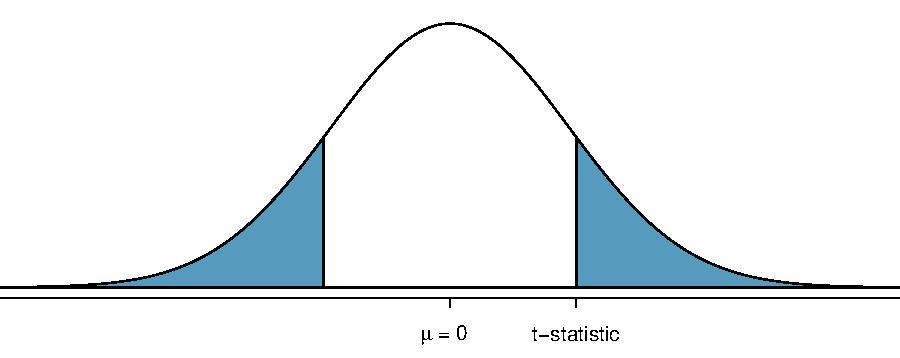
\includegraphics[width=0.9\textwidth]{ch_inference_foundations_oi_biostat/figures/pValueTwoSided/pValueTwoSided}
	\caption{A two-sided $p$-value for $H_A: \mu \neq \mu_0$ on a standard normal distribution. The shaded regions represent observations as or more extreme than $\overline{x}$ in either direction.}
	\label{pValueTwoSided}
\end{figure}

For one-sided tests with $H_A: \mu > \mu_0$, the $p$-value is given by $P(Z \geq t)$, as shown in Figure~\ref{pValueOneSided}. If $H_A: \mu < \mu_0$, the $p$-value is the area to the left of the $t$-statistic, $P(Z \leq t)$.

\begin{figure}[h]
	\centering
	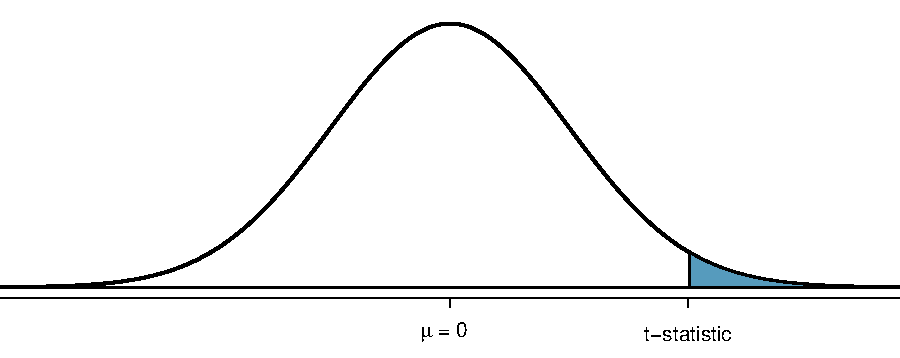
\includegraphics[width=0.9\textwidth]{ch_inference_foundations_oi_biostat/figures/pValueOneSided/pValueOneSided}
	\caption{A one-sided $p$-value for $H_A: \mu > \mu_0$ on a standard normal distribution is represented by the shaded area to the right of the $t$-statistic. This area equals the probability of making an observation as or more extreme than $\overline{x}$, if the null hypothesis is true.}
	\label{pValueOneSided}
\end{figure}


The $p$-value can either be calculated from software or from the normal probability tables. For the weight-difference example, the $p$-value is vanishingly small: $p = P(Z \leq - 4.22) + P(Z > 4.22)< 0.001$.

\subsubsection{Step 5: Drawing a conclusion}

To reach a conclusion about the null hypothesis, directly compare $p$ and $\alpha$. Note that for a conclusion to be informative, it must be presented in the context of the original question; it is not useful to only state whether or not $H_0$ is rejected.

If $p > \alpha$, the observed sample mean is not extreme enough to warrant rejecting $H_0$; more formally stated, there is insufficient evidence to reject $H_0$. A high $p$-value suggests that the difference between the observed sample mean and $\mu_0$ can reasonably be attributed to random chance.

If $p \leq \alpha$, there is sufficient evidence to reject $H_0$ and accept $H_A$. In the \data{cdc.samp} weight-difference data, the $p$-value is very small, with the $t$-statistic lying to the right of the population mean. The chance of drawing a sample with mean as large or larger than 18.2 if the distribution were centered at 0 is less than 0.001. Thus, the data support the conclusion that on average, the difference between actual and desired weight is  not 0 and is positive; people generally seem to feel they are overweight.

\begin{exercise}
  Suppose that the mean weight difference in the sampled group of 60 adults had been 7 pounds instead of 18.2 pounds, but with the same standard deviation of 33.46 pounds. Would there still be enough evidence at the $\alpha = 0.05$ level to reject $H_0: \mu = 0$ in favor of $H_A: \mu \neq 0$?\footnote{Re-calculate the $t$-statistic: $(7 - 0)/(33.46/\sqrt{60}) = 1.62$. The $p$-value $ P(Z \leq -1.62) + P(Z \geq 1.62) = 0.105$. Since $p$ > $\alpha$, there is insufficient evidence to reject $H_0$. In this case, a sample average difference of 7 is not large enough to discount the possibility that the observed difference is due to sampling variation, and that the observations are from a distribution centered at 0.}

\end{exercise}

\subsection{Two examples}


\begin{example}
{While fish and other types of seafood are important for a healthy diet, nearly all fish and shellfish contain traces of mercury. Dietary exposure to mercury can be particularly dangerous for young children and unborn babies. Regulatory organizations such as the US Food and Drug Administration (FDA) provide guidelines as to which types of fish have particularly high levels of mercury and should be completely avoided by pregnant women and young children; additionally, certain species known to have low mercury levels are recommended for consumption. While there is no international standard that defines excessive mercury levels in saltwater fish species, general consensus is that fish with levels above 0.50 parts per million (ppm) should not be consumed. A study conducted to assess mercury levels for saltwater fish caught off the coast of New Jersey found that a sample of 23 bluefin tuna had mean mercury level of 0.52 ppm, with standard deviation 0.16 ppm.\footnote{J. Burger, M. Gochfeld, Science of the Total Environment 409 (2011) 1418–1429} Based on these data, should the FDA add bluefin tuna from New Jersey to the list of species recommended for consumption, or should a warning be issued about their mercury levels?}
\label{hypTestTuna}

Let $\mu$ be the population average mercury content for bluefin tuna caught off the coast of New Jersey. Conduct a two-sided test of the hypothesis $\mu = 0.50$ ppm in order to assess the evidence for either definitive safety or potential danger.

\textit{Formulate the null and alternative hypotheses}. $H_0: \mu = 0.50$ ppm vs. $H_A: \mu \neq 0.50$ ppm

\textit{Specify the significance level, $\alpha$}.  A significance level of $\alpha = 0.05$ seems reasonable. 

\textit{Calculate the test statistic}. The  $t$-statistic has value
\begin{align*}
t &= \frac{\overline{x}-\mu_0}{s/\sqrt{n}} = \frac{0.53 - 0.50} {0.16/\sqrt{23}} = 0.859.
\end{align*}

\textit{Calculate the $p$-value}.

For this two-sided alternative $H_A: \mu \neq 0.50$, the $p$-value is 

\[P(Z \leq -t) + P(Z \geq t)= 2 \times P(Z \geq 0.859) = 0.390.\]

\begin{figure}[h]
	\centering
	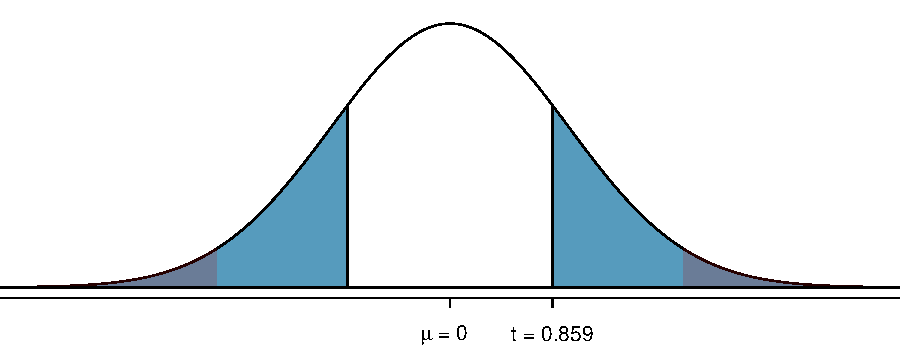
\includegraphics[width=0.8\textwidth]{ch_inference_foundations_oi_biostat/figures/pValueTuna/pValueTuna}
	\caption{The blue shaded region represents the $p$-value, the area to the right of $t = 0.859$ and to the left of $-t = -0.859$. The grey shaded region represents the \term{rejection region} as defined by $\alpha$; in this case, an area of 0.025 in each tail. The $t$-statistic calculated from $\overline{x}$ would have to lie within either of the grey regions in order to constitute sufficient evidence against the null hypothesis.}
	\label{pValueTuna}
\end{figure}

\textit{Draw a conclusion}. The $p$-value is larger than the specified significance level $\alpha$, as shown in Figure~\ref{pValueTuna}.\footnote{The grey shaded regions are bounded by -1.96 and 1.96, since the area within 1.96 standard deviations of the mean captures 95\% of the distribution.} The data do not show that the mercury content of bluefin tuna caught off the coast of New Jersey differs significantly from 0.50 ppm. Since $p > \alpha$, there is insufficient evidence to reject the null hypothesis that the mean mercury level for the New Jersey coastal population of bluefin tuna is 0.50 ppm. 

Note that "failure to reject" is not equivalent to "accepting" the null hypothesis. Recall the earlier analogy related to the principle of "innocent until proven guilty". If there is not enough evidence to prove that the defendant is guilty, the official decision must be "not guilty", since the defendant may not necessarily be innocent. Similarly, while there is not enough evidence to suggest that $\mu$ is not equal to 0.5 ppm, it would be incorrect to claim that the evidence states that $\mu$ \textit{is} 0.5 ppm.

From these data, there is not statistically significant evidence to either recommend these fish as clearly safe for consumption or to warn consumers against eating them. Based on these data, the Food and Drug Administration might decide to monitor this species more closely and conduct further studies. 

\end{example}

%\newpage

\begin{example}
{In 2015, the National Sleep Foundation published new guidelines for the amount of sleep recommended for adults: 7-9 hours of sleep per night.\footnote{Sleep Health: Journal of the National Sleep Foundation, Vol. 1, Issue 1, pp. 40 - 43} The NHANES survey includes a question asking respondents about how many hours per night they sleep; the responses are available in \data{nhanes.samp}. In the sample of 134 adults used in the BMI example, the average reported hours of sleep is 6.90, with standard deviation 1.39. Is there evidence that American adults sleep less than 7 hours per night?}

Let $\mu$ be the population average of hours of sleep per night for US adults. Conduct a one-sided test, since the question asks whether the average amount of sleep per night might be less than 7 hours. 

\textit{Formulate the null and alternative hypotheses}. $H_0: \mu = 7$ hours vs. $H_A: \mu < 7$ hours

\textit{Specify the significance level, $\alpha$}.  Let $\alpha = 0.05$, since the question does not reference a different value. 

\textit{Calculate the test statistic}. The $t$-statistic has value
\[t = \frac{\overline{x}-\mu_0}{s/\sqrt{n}} = \frac{6.90 - 7.00} {1.33/\sqrt{134}} = -0.864.\]

\textit{Calculate the $p$-value}.

For this one-sided alternative $H_A: \mu < 7$, the $p$-value is 

\[P(Z \leq t) = P(Z < -0.864) = 0.19.\]

Since the alternative states that $\mu_0$ is less than 7, the $p$-value is represented by the area to the left of $t = -0.864$, as shown in Figure~\ref{pValueSleep}.


\begin{figure}[h]
	\centering
	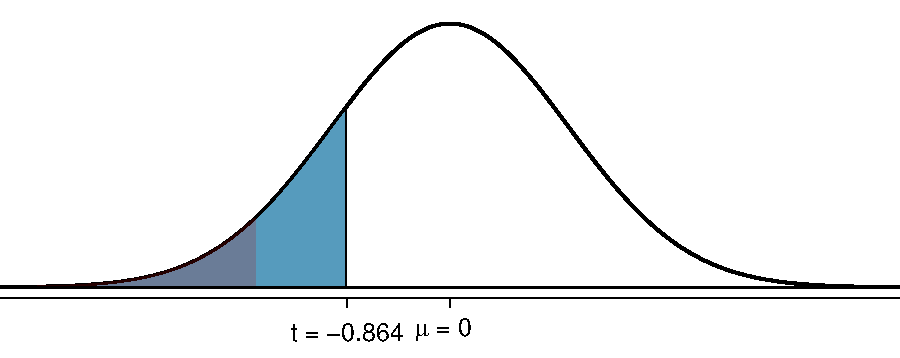
\includegraphics[width=0.8\textwidth]{ch_inference_foundations_oi_biostat/figures/pValueSleep/pValueSleep}
	\caption{The blue shaded region represents the $p$-value, the area to the left of $t = -0.864$. The grey shaded region represents the rejection region of area 0.05 in the left tail.}
	\label{pValueSleep}
\end{figure}

\textit{Draw a conclusion}.  The $p$-value is larger than the specified significance level $\alpha$. The null hypothesis is not rejected since the data do not represent sufficient evidence to support the claim that American adults sleep less than 7 hours per night.

\end{example}

\begin{exercise}
	From these data, is there sufficient evidence at the $\alpha = 0.10$ significance level to support the claim that American adults sleep more than 7 hours per night?\footnote{The $t$-statistic does not change from 1.65. Re-calculate the $p$-value since the alternative hypothesis is now $H_A: \mu > 7$: $P(Z \geq -0.864) = 0.81$. Since $p$ > $\alpha$, there is insufficient evidence to reject $H_0$ at $\alpha = 0.10$. A common error when conducting one-sided tests is to assume that the $p$-value will always be the area in the smaller of the two tails to the right or left of the observed value. It is important to remember that the area corresponding to the $p$-value is in the direction specified by the alternative hypothesis.\\
	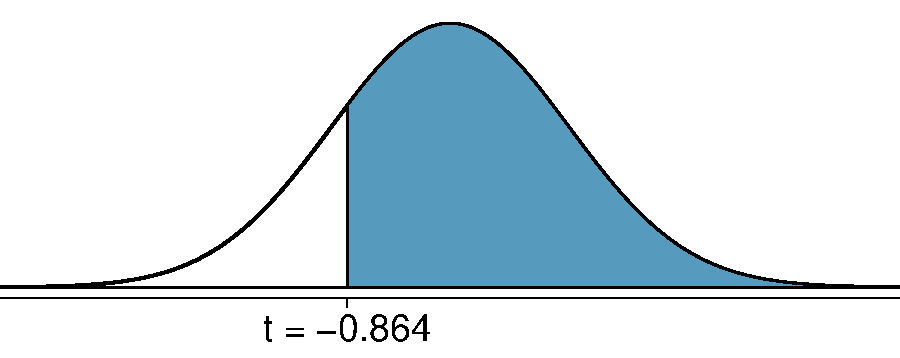
\includegraphics[width=0.3\textwidth]{ch_inference_foundations_oi_biostat/figures/pValueSleep/pValueSleepEx}}
\end{exercise}

\subsection{Hypothesis testing and confidence intervals}

The relationship between a hypothesis test and the corresponding confidence interval is defined by the significance level $\alpha$; the two approaches are based on the same inferential logic, and differ only in perspective. The hypothesis testing approach asks whether $\overline{x}$ is far enough away from $\mu_0$ to be considered extreme, while the confidence interval approach asks whether $\mu_0$ is close enough to $\overline{x}$ to be plausible. In both cases, "far enough" and "close enough" are defined by $\alpha$, which determines the $t^{\star}$ used to calculate the margin of error $m = t^{\star} (s/\sqrt{n}) $.\footnote{If the normal distribution is used, then $m = z^{\star} (s/\sqrt{n})$.}

\begin{list}{}{}
	\item \textit{Hypothesis Test}. For a two-sided test,  $\overline{x}$ needs to be at least $m$ units away from $\mu_0$ in either direction to be considered extreme. The $t$-points marking off the rejection region are equal to the $t^\star$ value used in the confidence interval, with the positive and negative $t$-points accounting for the $\pm$ structure in the confidence interval.
	
	\item \textit{Confidence Interval}. The plausible range of values for $\mu_0$ around $\overline{x}$ is defined as $(\overline{x} - m, \ \overline{x} + m)$. If $\mu_0$ is plausible, it can at most be $m$ units away in either direction from $\overline{x}$. If the interval does not contain $\mu_0$, then $\mu_0$ is implausible according to $\alpha$ and there is sufficient evidence to reject $H_0$.
\end{list}

Suppose that a two-sided test is conducted at significance level $\alpha$; the confidence level of the matching interval is ($1 - \alpha$)\%. For example, a two-sided hypothesis test with $\alpha = 0.05$ can be compared to a 95\% confidence interval. A hypothesis test will reject at $\alpha = 0.05$ if the 95\% confidence interval does not contain the null hypothesis value of the population mean ($\mu_0$).

\begin{termBox}{\tBoxTitle{The relationship between two-sided hypothesis tests and confidence intervals}
{When testing the null hypothesis $H_0:\mu = \mu_0$ against the two-sided alternative $H_A: \mu \neq \mu_0$, $H_0$ will be rejected at significance level $\alpha$ when the $100(1-\alpha)\%$ confidence interval for $\mu$ does not contain $\mu_0$. }}
\end{termBox}

\begin{example}
{Calculate the confidence interval for the average mercury level for bluefin tuna caught off the coast of New Jersey. The summary statistics for the sample of 21 fish are $\overline{x} = 0.53$ ppm and $s = 0.16$ ppm. Does the interval agree with the results of Example~\ref{hypTestTuna}?}

The 95\% confidence interval is: 

\[\overline{x} \pm 1.96 \dfrac{s}{\sqrt{n}}= 0.53 \pm 1.96 \frac{0.16}{\sqrt{21}} = (0.462, 0.598) \text{ ppm}.\]

The confidence interval is relatively wide, containing values below 0.50 ppm that might be regarded as safe, in addition to values that might be regarded as potentially dangerous. This interval supports the conclusion reached from hypothesis testing; the sample data does not suggest that the mercury level differs significantly from 0.50 ppm in either direction. 

\end{example}
	
The same relationship applies for one-sided hypothesis tests. For example, a one-sided hypothesis test with $\alpha = 0.05$ and $H_A: \mu > \mu_0$ corresponds to a one-sided 95\% confidence interval that has a lower bound, but no upper bound (i.e., ($\overline{x} - m, \infty$)).
	
\begin{termBox}{\tBoxTitle{The relationship between one-sided hypothesis tests and confidence intervals}
  {
  	\begin{itemize}
	\item When testing the null hypothesis $H_0:\mu = \mu_0$ against the one-sided alternative $H_A: \mu > \mu_0$, $H_0$ will be rejected at significance level $\alpha$ when $\mu_0$ is smaller than the lower bound of the $100(1-\alpha)\%$ confidence interval for $\mu$. This is equivalent to $\mu_0$ having a value outside the lower one-sided confidence interval ($\overline{x} - m, \infty$).

	\item When testing the null hypothesis $H_0:\mu = \mu_0$ against the one-sided alternative $H_A: \mu < \mu_0$, $H_0$ will be rejected at significance level $\alpha$ whenever $\mu_0$ is larger than the upper bound of the $100(1-\alpha)\%$ confidence interval for $\mu$. This is equivalent to $\mu_0$ having a value outside the upper one-sided confidence interval ($-\infty, \overline{x} + m$).
	\end{itemize}
  }}
\end{termBox}
		
\begin{example}
{Previously, a hypothesis test was conducted at $\alpha = 0.05$ to test the null hypothesis $H_0: \mu = 7$ hours against the alternative $H_A: \mu < 7$ hours, for the average sleep per night US adults. Calculate the corresponding one-sided confidence interval and compare the information obtained from a confidence interval versus a hypothesis test. The summary statistics for the sample of 134 adults are $\overline{x} = 6.9$ and $s = 1.39$.}	

In theory, a one-sided upper confidence interval extends to $\infty$ on the left side, but since it is impossible to get negative sleep, it is more sensible to bound this confidence interval by 0.  The upper one-sided 95\% confidence interval is

\[(0, \overline{x} + 1.645 \dfrac{s}{\sqrt{n}}) = (0, 6.9 + 1.645\dfrac{1.39}{\sqrt{134}}) = (0, \ 7.1)\text{ hours.} \]

From these data, we can be 95\% confident that the average sleep per night among US adults is at most 7.1 hours per night. The $\mu_0$ value of 7 hours is inside the one-sided interval; thus, there is not sufficient evidence to reject the null hypothesis $H_0: \mu = 7$ against the one-sided alternative $H_0: \mu < 7$ hours at $\alpha = 0.05$. 

The interval provides a range of plausible values for a parameter based on the observed sample; in this case, the data suggest that the population average sleep per night for US adults is no larger than 7.1 hours. The $p$-value from a hypothesis test represents a measure of the strength of the evidence against the null hypothesis, indicating how unusual the observed sample would be under $H_0$; the hypothesis test indicated that the data do not seem extreme enough ($p = 0.19$) to contradict the hypothesis that the population average sleep hours per night is 7. 

In practice, both a $p$-value and a confidence interval are computed when using a sample to make inferences about a population parameter.

\end{example}

\subsection{Decision errors}

Hypothesis tests can potentially result in incorrect decisions, such as rejecting the null hypothesis when the null is actually true. Table~\ref{fourHTScenarios} shows the four possible ways that the conclusion of a test can be right or wrong.

\begin{table}[ht]
	\centering
	\begin{tabular}{l l c c}
		& & \multicolumn{2}{c}{\textbf{Test conclusion}} \\
		\cline{3-4}
		\vspace{-3.7mm} \\
		& & Fail to reject $H_0$ &  Reject $H_0$ in favor of $H_A$ \\
		\cline{2-4}
		\vspace{-3.7mm} \\
		& $H_0$ True & Correct Decision &  Type~1 Error \\
		\raisebox{1.5ex}{\textbf{Reality}} & $H_A$ True & Type~2 Error & Correct Decision\\
		\cline{2-4}
	\end{tabular}
	\caption{Four different scenarios for hypothesis tests.}
	\label{fourHTScenarios}
\end{table}

Rejecting the null hypothesis when the null is true represents a \term{Type I error}, while a \term{Type II error} refers to failing to reject the null hypothesis when the alternative is true. 

\begin{example}
{In a trial, the defendant is either innocent ($H_0$) or guilty ($H_A$). After hearing evidence from both the prosecution and the defense, the court must reach a verdict. What does a Type~I Error represent in this context? What does a Type~II Error represent?}	
If the court makes a Type~I error, this means the defendant is innocent, but wrongly convicted (rejecting $H_0$ when $H_0$ is true). A Type~II error means the court failed to convict a defendant that was guilty (failing to reject $H_0$ when $H_0$ is false).		
\label{whatAreTheErrorTypesInUSCourts}	
\end{example}

The probability of making a Type I error is the same as the significance level $\alpha$, since $\alpha$ determines the cutoff point for rejecting the null hypothesis. For example, if $\alpha$ is chosen to be 0.05, then there is a 5\% chance of incorrectly rejecting $H_0$. 

The rate of Type I error can be reduced by lowering $\alpha$ (e.g., to 0.01 instead of 0.05); doing so requires an observation to be more extreme to qualify as sufficient evidence against the null hypothesis. However, this inevitably raises the rate of Type II errors, since the test will now have a higher chance of failing to reject the null hypothesis when the alternative is true.

\begin{example}
{In a courtroom setting, how might the rate of Type I errors be reduced? What effect would this have on the rate of Type II errors?}	
Lowering the rate of Type I error is equivalent to raising the standards for conviction such that fewer people are wrongly convicted. This increases Type II error, since higher standards for conviction leads to fewer convictions for people who are actually guilty.
\end{example}


\begin{exercise} \label{howToReduceType2ErrorsInUSCourts}
	In a courtroom setting, how might the rate of Type II errors be reduced? What effect would this have on the rate of Type I errors?\footnote{To lower the rate of Type II error, the court could lower the standards for conviction, or in other words, lower the bar for what constitutes sufficient evidence of guilt (increase $\alpha$, e.g. to 0.10 instead of 0.05). This will result in more guilty people being convicted, but also increase the rate of wrongful convictions, increasing the Type I error.}
\end{exercise}

\index{hypothesis testing!decision errors|)}

\subsubsection{Choosing a significance level}

\index{hypothesis testing!significance level|(}
\index{significance level|(}

Reducing the error probability of one type of error increases the chance of making the other type. As a result, the significance level is often adjusted based on the consequences of any decisions that might follow from the result of a significance test.

\label{significanceLevel}

By convention, most scientific studies use a significance level of $\alpha = 0.05$; small enough such that the chance of a Type I error is relatively rare (occurring on average 5 out of 100 times), but also large enough to prevent the null hypothesis from almost never being rejected. If a Type I error is especially dangerous or costly, a smaller value of $\alpha$ is chosen (e.g., 0.01). Under this scenario, it is better to be cautious about rejecting the null hypothesis, so very strong evidence against $H_0$ is required in order to reject the null and accept the alternative. Conversely, if a Type II error is relatively dangerous, then a larger value of $\alpha$ is chosen (e.g., 0.10). Hypothesis tests with larger values of $\alpha$ will reject $H_0$ more often.

For example, in the early stages of assessing a drug therapy, it may be important to continue further testing even if there is not very strong initial evidence for a beneficial effect. If the scientists conducting the research know that any initial positive results will eventually be more rigorously tested in a larger study, they might choose to use $\alpha = 0.10$ to reduce the chances of making a Type II error: prematurely ending research on what might turn out to be a promising drug.

A government agency responsible for approving drugs to be marketed to the general population, however, would likely be biased towards minimizing the chances of making a Type I error\textemdash approving a drug that turns out to be unsafe or ineffective. As a result, they might conduct tests at significance level 0.01 in order to reduce the chances of concluding that a drug works when it is in fact ineffective. The US FDA and the European Medical Agency (EMA) customarily require that two independent studies show the efficacy of a new drug or regimen using $\alpha = 0.05$, though other values are sometimes used.

\index{significance level|)}
\index{hypothesis testing!significance level|)}
\index{hypothesis testing|)}

\subsection{Choosing between one-sided and two-sided tests}

In some cases, the choice of a one-sided or two-sided test can influence whether the null hypothesis is rejected. For example, consider a sample for which the $t$-statistic is 1.80. If a two-sided test is conducted at $\alpha = 0.05$, the $p$-value is

\[P(Z \leq -t) + P(Z \geq t)= 2P(Z \geq 1.80) = 0.072.\]

There is insufficient evidence to reject $H_0$, since $p > \alpha$. However, what if a one-sided test is conducted at $\alpha = 0.05$, with $H_A: \mu > \mu_0$? In this case, the $p$-value is

\[P(Z \geq t)= P(Z \geq 1.80) = 0.036.\]

The conclusion of the test is different: since $p < \alpha$, there is sufficient evidence to reject $H_0$ in favor of the alternative hypothesis. Figure~\ref{twoSidedTestConservative} illustrates the different outcomes from the tests.

\begin{figure}[h]
	\centering
	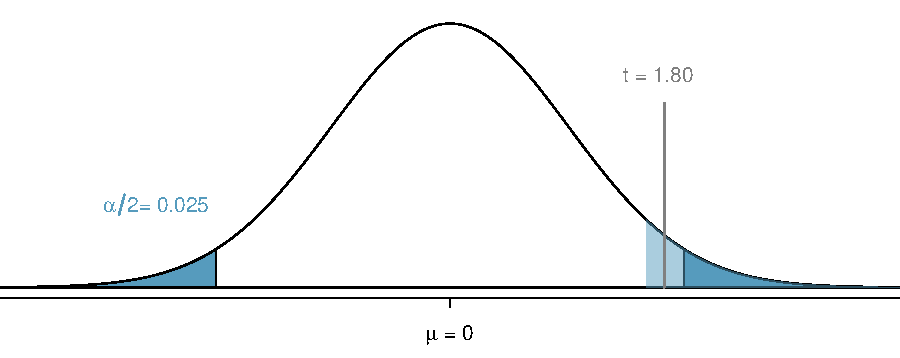
\includegraphics[width=0.9\textwidth]
	{ch_inference_foundations_oi_biostat/figures/twoSidedTestConservative/twoSidedTestConservative}
	\caption{Under a one-sided test at significance level $\alpha$ = 0.05, a $t$-statistic of 1.80 is within the rejection region (shaded light blue). However, it would not be within the rejection region under a two-sided test with $\alpha$ = 0.05 (darker blue).}
	\label{twoSidedTestConservative}
\end{figure}

Two-sided tests are more "conservative" than one-sided tests; it is more difficult to reject the null hypothesis with a two-sided test. The $p$-value for a one-sided test is exactly half the $p$-value for a two-sided test conducted at the same significance level; as a result, it is easier for the $p$-value from a one-sided test to be smaller than $\alpha$. Additionally, since the rejection region for a two-sided test is divided between two tails, a test statistic needs to be more extreme in order to fall within a rejection region. While the $t$-statistic of 1.80 is not within the two-sided rejection region, it is within the one-sided rejection region.\footnote{The two-sided rejection regions are bounded by -1.96 and 1.96, while the one-sided rejection region begins at 1.65.}

For a fixed sample size, a one-tailed test will have a smaller probability of Type II error in comparison to a two-tailed test conducted at the same $\alpha$ level. In other words, with a one-sided test, it is easier to reject the null hypothesis if the alternative is actually true. 

The choice of test should be driven by context, although it is not always clear which test is appropriate. Since it is easier to reject $H_0$ with the one-tailed test, it might be tempting to always use a one-tailed test when a significant result in a particular direction would be interesting or desirable. 

However, it is important to consider the potential consequences of missing a significant difference in the untested direction. Generally, a two-sided test is the safest option, since it does not incorporate any existing biases about the direction of the results and can detect a difference at either the upper or lower tail. In the 1980s, researchers were interested in assessing a new set of drugs expected to be more effective at reducing heart arrhythmias than previously available therapies. They designed a one-sided clinical trial, convinced that the newer therapy would reduce mortality. The trial was quickly terminated due to an unanticipated effect of the drug; an independent review board found that the newer therapy was almost 4 times as likely to kill patients as a placebo! In a clinical research setting, it can be dangerous and even unethical to conduct a one-sided test under the belief that there is no possibility of patient harm from the drug intervention being tested.

%cite two_tailed_clinical

One-sided tests are appropriate if the consequences of missing an effect in the untested direction are negligible, or if a large observed difference in the untested direction and a conclusion of "no difference" lead to the same decision. For example, suppose that a company has developed a drug to reduce blood pressure that is cheaper to produce than current options available on the market. If the drug is shown to be equally effective or more effective than an existing drug, the company will continue investing in it. Thus, they are only interested in testing the alternative hypothesis that the new drug is less effective than the existing drug, in which case, they will stop the project. It is acceptable to conduct a one-sided test in this situation since missing an effect in the other direction causes no harm. 

The decision as to whether to use a one-sided or two-sided test must be made before data analysis begins, in order to avoid biasing conclusions based on the results of a hypothesis test. In particular, changing to a one-sided test after discovering that the results are "almost" significant for the two-sided test is unacceptable. Manipulating analyses in order to achieve low $p$-values leads to invalid results that are often not replicable. Unfortunately, this kind of "significance-chasing" has become widespread in published science, leading to concern that most current published research findings are false.

%cite statistical_errors

%cite published_research_false

% edits to here 24 jul 2017

\subsection{The informal use of $p$-values}
\label{informalUseOfp-values}

Formal hypothesis tests are designed for settings where a decision or a claim about a hypothesis follows a test, such as in scientific publications where an investigator wishes to claim that an intervention changes an outcome.  However, progress in science is usually based on a collection of studies or experiments, and it is often the case that the results of one study are used as a guide for the next study or experiment. 

Sir Ronald Fisher was the first to propose using $p$-values as one of the statistical tools for evaluating an experiment.  In his view, an outcome from an experiment that would only happen 1 in 20 times ($p$ = 0.05) was worth investigating further. The use of $p$-values for formal decision making came later.  While valuable, formal hypothesis testing can often be overused; not all significant results should lead to a definitive claim, but instead prompt further analysis.

The formal use of p-values is emphasized here because of its prominence in the scientific literature, and because the steps outlined are fundamental to the scientific method for empirical research: specify hypotheses, state in advance how strong the evidence should be to constitute sufficient evidence against the null, specify the method of analysis and compute the test statistic, draw a conclusion. These steps are designed to avoid the pitfall of choosing a hypothesis or method of analysis that is biased by the data and hence reaches a conclusion that may not be reproducible.


\section{Notes}
\label{ch4Summary}

Confidence intervals and hypothesis testing are two of the central concepts in inference for a population based on a sample. The confidence interval shows a range of population parameter values consistent with the observed sample, and is often used to design additional studies. Hypothesis testing is a useful tool for evaluating the strength of the evidence against a working hypothesis according to a pre-specified standard for accepting or rejecting hypotheses.

The calculation of $p$-values and confidence intervals is relatively straightforward; given the necessary summary statistics, $\alpha$, and confidence coefficients, finding any $p$-value or confidence interval simply involves a set of formulaic steps. However, the more difficult parts of any inference problem are the steps that do not involve any calculations. Specifying appropriate null and alternative hypotheses for a test relies on an understanding of the problem context and the scientific setting of the investigation. Similarly, a choice about a confidence coefficient for an interval relies on judgment as to balancing precision against the chance of possible error. It is also not necessarily obvious when a significance level other than $\alpha = 0.05$ should be applied. These choices represent the largest distinction between a true statistics problem as compared to a purely mathematical exercise. 

Furthermore, in order to rely on the conclusions drawn from making inferences, it is necessary to consider factors such as study design, measurement quality, and the validity of any assumptions made. For example, is it valid to use the normal approximation to calculate $p$-values? In small to moderate sample sizes ($30 \leq n \leq 50$), it may not be clear that the normal model is accurate. It is even necessary to be cautious about the use and interpretation of the $p$-value. For example, an article published in \textit{Nature} about the mis-use of $p$-values references a published study that showed people who meet their spouses online are more likely to have marital satisfaction, with $p$-value less than 0.001. However, statistical significance does not measure the importance or practical relevance of a result; in this case, the change in happiness moved from 5.48 to 5.64 on a 7-point scale. A $p$-value reported without context or other evidence is uninformative and potentially deceptive.

%cite statistical_errors and asa_p_values

These nuanced issues cannot be adequately covered in any introduction to statistics. It is unrealistic to encourage students to use their own judgment with aspects of inference that even experienced investigators find challenging. At the same time, it would also be misleading to suggest that the choices are always clear-cut in practice. It seems best to offer some practical guidance for getting started:

\begin{itemize}
	\item The default choice of $\alpha$ is 0.05; similarly, the default confidence coefficient for a confidence interval is 95\%. 
	
	\item Unless it is clear from the context of a problem that change in only one direction from the null hypothesis is of interest, the alternative hypothesis should be two-sided.
	
	\item The use of a standard normal distribution to calculate $p$-values is reasonable for sample sizes of 30 or more if the distribution of data are not strongly skewed and there are no large outliers. If there is skew or a few large outliers, sample sizes of 50 or more are usually sufficient.\footnote{With the use of statistical computing software, it is often simpler to always use the $t$-distribution, which is valid for any sample size.}
	
	\item Pay attention to the context of a problem, particularly when formulating hypotheses and drawing conclusions.
\end{itemize}

The next chapters will discuss methods of inference in specific settings, such as comparing two groups. These settings expand on the concepts discussed in this chapter and offer additional opportunities to practice calculating tests and intervals, reading problems for context, and checking underlying assumptions behind methods of inference.



